%%%%%%%%%%%%%%%%%%%%%%%%%%%%%%%%%%%%%%%%%%%%%%%%%%%%%%%%%%%%
%%% ELIFE ARTICLE TEMPLATE
%%%%%%%%%%%%%%%%%%%%%%%%%%%%%%%%%%%%%%%%%%%%%%%%%%%%%%%%%%%%
%%% PREAMBLE 
\documentclass[9pt,lineno]{elife}
% Use the onehalfspacing option for 1.5 line spacing
% Use the doublespacing option for 2.0 line spacing
% Please note that these options may affect formatting.

\usepackage{lipsum} % Required to insert dummy text
\usepackage[version=4]{mhchem}
\usepackage{siunitx}
\DeclareSIUnit\Molar{M}
\usepackage{indentfirst} %I prefer to have indents following section headings, I find it to be more consistent in style throughout document

\renewcommand{\floatpagefraction}{1}

%%%%%%%%%%%%%%%%%%%%%%%%%%%%%%%%%%%%%%%%%%%%%%%%%%%%%%%%%%%%
%%% ARTICLE SETUP
%%%%%%%%%%%%%%%%%%%%%%%%%%%%%%%%%%%%%%%%%%%%%%%%%%%%%%%%%%%%
\title{Transcriptional dynamics of influenza virus infection in single cells}

\author[1]{Alistair B. Russell}
\author[2]{Cole Trapnell}
\author[1,2*]{Jesse D. Bloom}
\affil[1]{Basic Sciences Division and Computational Biology Program, Fred Hutchinson Cancer Research Center, Seattle, United States}
\affil[2]{Department of Genome Sciences, University of Washington, Seattle, United States}
\corr{jbloom@fredhutch.org}{}

% \presentadd[\authfn{5}]{eLife Sciences editorial Office, eLife Sciences, Cambridge, United Kingdom}

%%%%%%%%%%%%%%%%%%%%%%%%%%%%%%%%%%%%%%%%%%%%%%%%%%%%%%%%%%%%
%%% ARTICLE START
%%%%%%%%%%%%%%%%%%%%%%%%%%%%%%%%%%%%%%%%%%%%%%%%%%%%%%%%%%%%

\begin{document}

\maketitle

\begin{abstract}
Influenza virus infection induces large changes in cellular transcription.
Previously this has mostly been looked at using bulk measurements
Here we examine the process at the level of single cells.
We find extremely wide variation in the extent of viral gene transcription across infected cells.
IFN induction is very rare.
Some cellular pathways may be consistently altered in cells with high burden of viral transcripts.
Overall, highlights remarkable heterogeneity in the outcome of infection.
\end{abstract}


\section{Introduction}

Heterogeneity is important in a lot of cellular processes even when isogenic~\citep{shalek2013single,shalek2014single}.

Population (genetic) heterogeneity is also important. 
Viral quasispecies, cancer single-cell, etc.
Salmonella paper (PhoP).

Literature on viral burst-size heterogeneity.
This goes back to Delbruck, Andino polio paper~\citep{schulte2014single}, the MDCK / flu paper.

Discuss segmented nature of influenza.
Maybe in the context of how this could further increase heterogeneity because there is a lot of potential for entire genes to be missing.
Includes Yewdell and Lowen papers.

\section{Results}

\subsection{Strategy to measure mRNA in single virus-infected cells.}
We performed single-cell mRNA sequencing using a droplet-based system that physically isolates individual cells prior to reverse transcription.
Each droplet is associated with a unique \emph{cell barcode} that tags all mRNAs from that cell during reverse-transcription.
A random \emph{unique molecular identifier (UMI)} is additionally appended to each mRNA molecule during reverse transcription.
The 3' ends of the mRNAs are sequenced and mapped to the human and influenza transcriptomes to determine the transcript identities.
This information is combined with that provided by the UMIs and cell barcodes to quantify the number of molecules of each mRNA species that have been captured for each cell.

Infected cells will express viral as well as cellular mRNAs, however the cell barcodes and UMIs cannot distinguish whether a cell was initially infected by one or multiple viral particles.
We therefore engineered an influenza virus (strain A/WSN/1933) that additionally carried \emph{viral barcodes} consisting of synonymous mutations near the 3' end of each transcript (Figure~\ref{fig:workflow}A).
Critically, these synonymous mutations did not greatly impact viral growth kinetics (Figure~\ref{fig:workflow}B).
We infected A549 human lung carcinoma cells with an equal mix of the wildtype and synonymously barcoded viruses.
Cells infected by a single virion will exclusively express mRNAs from either wild-type or synonymously barcoded virus, whereas cells that are co-infected with multiple virions will often express mRNAs from both the wildtype and synonymously barcoded viruses (Figure~\ref{fig:workflow}C).
\begin{figure}
\centerline{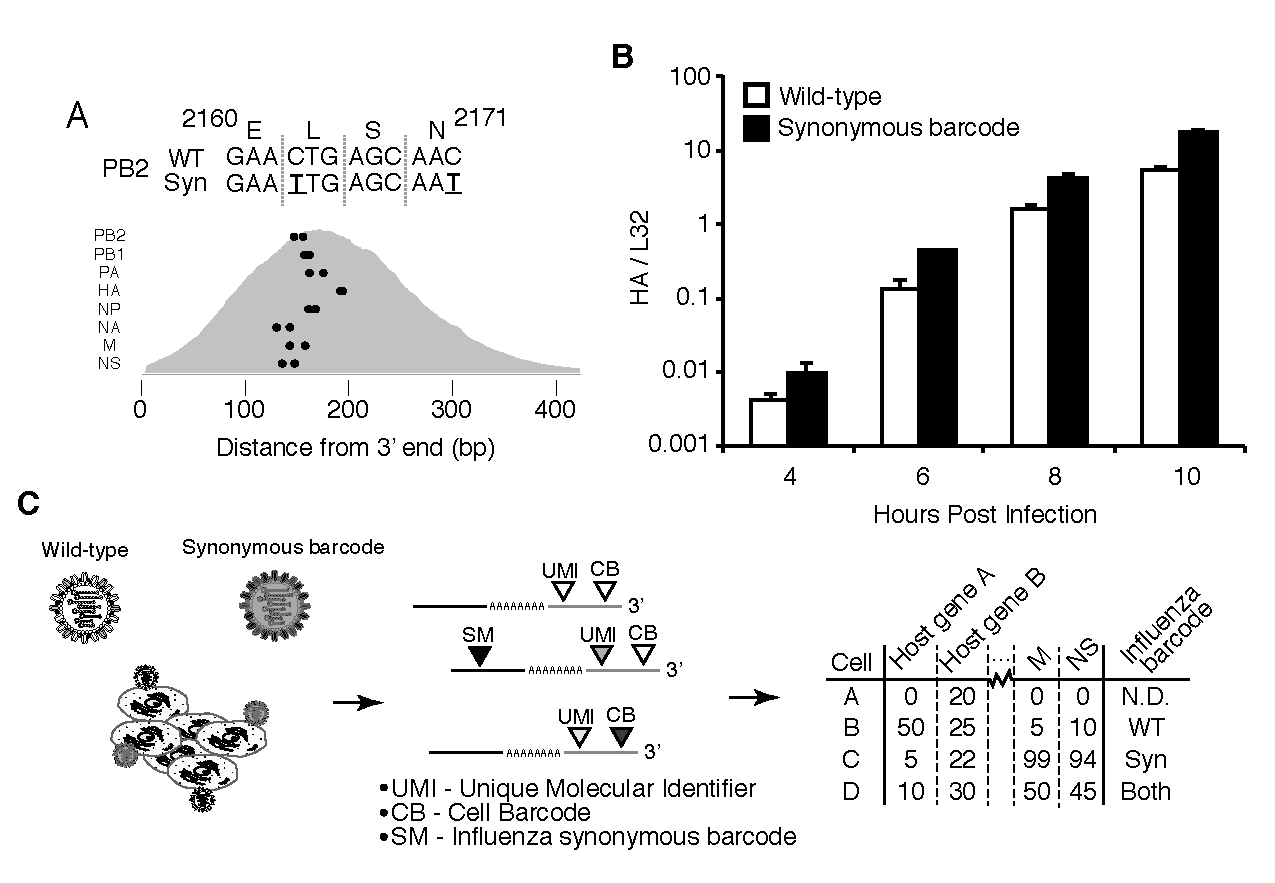
\includegraphics[width=0.8\linewidth]{figures/Workflow/workflow.pdf}}
\caption{\label{fig:workflow} Experimental design.
{\bf (A)}  
We engineered a virus that carried two synonymous mutations near the 3' end of each mRNA.
At top are the specific mutations for the PB2 gene.
At bottom are locations of the synonymous mutations relative to the typical distribution of read depth for the 3'-end sequencing of the mRNA.
{\bf (B)} 
The wild-type and synonymously barcoded viruses transcribe their genes with similar kinetics. 
Shown is the abundance of the viral hemagglutinin (HA) transcript relative to the cellular housekeeping gene L32 as assessed by qPCR in A549 cells infected at an MOI of 0.5 (as determined on MDCK-SIAT1 cells).
{\bf (C)}  
A549 cells were infected with an equal mixture of mutant and wild-type virus. 
Immediately prior to sequencing, cells were physically separated into droplets and cDNA libraries were generated containing the indicated barcodes. 
The libraries were deep sequenced, and the data processed to create a matrix that gives the number of molecules of each transcript observed in each cell.
Infected cells were further annotated by whether their viral mRNAs derived from wildtype virus, synonymously barcoded virus, or both.
Abbreviations: WT -- wild-type, Syn -- Synonymous Barcode.
}
\figdata{Sequences of wild-type and barcoded viruses are in \texttt{viralsequences.fasta}.}
\end{figure}

We also took care to generate stocks of virus that were relatively ``pure'' of defective particles.
Stocks of viruses typically contain an array of biologically active viral particles, some of which are defective for replication owing to mutations or deletions in essential viral genes.
These defective particles become prevalent when a virus is grown at high multiplicity of infection (MOI), where complementation permits the growth of otherwise deleterious genotypes.
To minimize the levels of defective particles, we propagated our viral stocks at low MOI for a relatively brief period of time~\citep{xue2016propagation}.
We then validated that our stocks exhibited greater purity of infectious particles than a stock propagated at high MOI by verifying that they had a higher ratio of infectious particles to both virion RNA (Figure~\ref{fig:viruspopulations}A) and particles capable of inducing expression of a single viral protein (Figure~\ref{fig:viruspopulations}B).
In addition, viral stocks with many defective particles are more immunostimulatory~\citep{tapia2013defective}.
We confirmed that our viral stocks induced much less interferon than a stock propagated at higher MOI (Figure~\ref{fig:viruspopulations}D).

\begin{figure}
\centerline{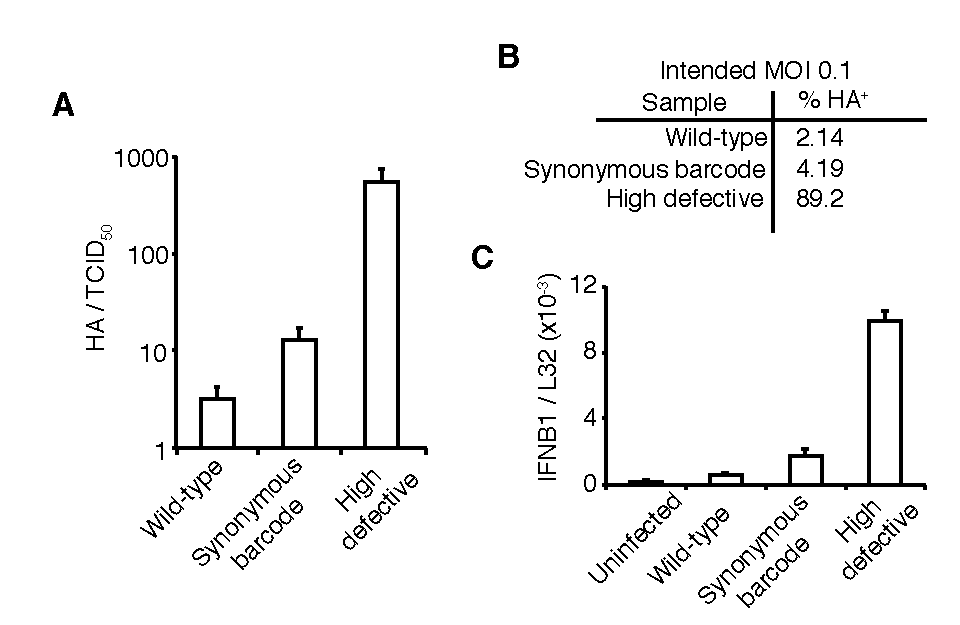
\includegraphics[width=0.7\linewidth]{figures/Validating_barcode_virus/validating_populations_D02.pdf}}
\caption{\label{fig:viruspopulations} The viral stocks in our experiments are relatively pure of defective particles. 
{\bf (A)}
Our viral stocks have a higher ratio of infectious particles to HA virion RNA compared to a high-defective stock propagated at high MOI.
HA viral RNA was quantified by qPCR on virions. 
{\bf (B)} 
Our viral stocks have a higher ratio of infectious particles to particles capable of expressing the viral HA protein.
A549 cells were infected with all three viral stocks at an MOI of 0.1, and the percentage of cells expressing HA protein at 9 hours post-infection was quantified by antibody staining and flow cytometry.
{\bf (C)} 
Our viral stocks are less immunostimulatory than virus propagated at high MOI. 
Measurements of \textit{IFNB1} transcript by qPCR normalized to the housekeeping gene L32 in A549 cells at 10 hours post infection at an MOI of 0.5.
MOIs were calculated by TCID50 on MDCK-SIAT1 cells.}
\figsupp[Flow cytometry data for calculating the percentage of HA-expressing cells.]{Longer caption}{\emph{HA-expression flow cytometry supplemental figure needs to be created.}}
\end{figure}

\subsection{Single cells show a wide range of expression of viral transcripts.}
We infected at low MOI with a mixture of the wildtype and synonymously barcoded viruses, and collected cells for sequencing at 6, 8, and 10 hours post-infection, including a replicate of the 8-hour timepoint.
We recovered between 3,000 and 4,000 cells for each sample (Figure~\ref{fig:cells}A). 
As expected for a low-MOI infection, most cells expressed little or no viral mRNA (Figure~\ref{fig:cells}B).
Also as expected, the amount of viral mRNA per cell among infected cells increased over time (Figure~\ref{fig:cells}B).
But what was most notable was how widely the number of viral mRNA molecules varied among infected cells.
While the fraction of mRNA derived from virus was $<$0.1\% for most infected cells, viral mRNA constituted close to half the transcriptome in a few cells at 8 and 10 hours (Figure~\ref{fig:cells}C).
Therefore, there is extraordinary variability in the number of viral transcripts per infected cell.

\begin{figure}
\centerline{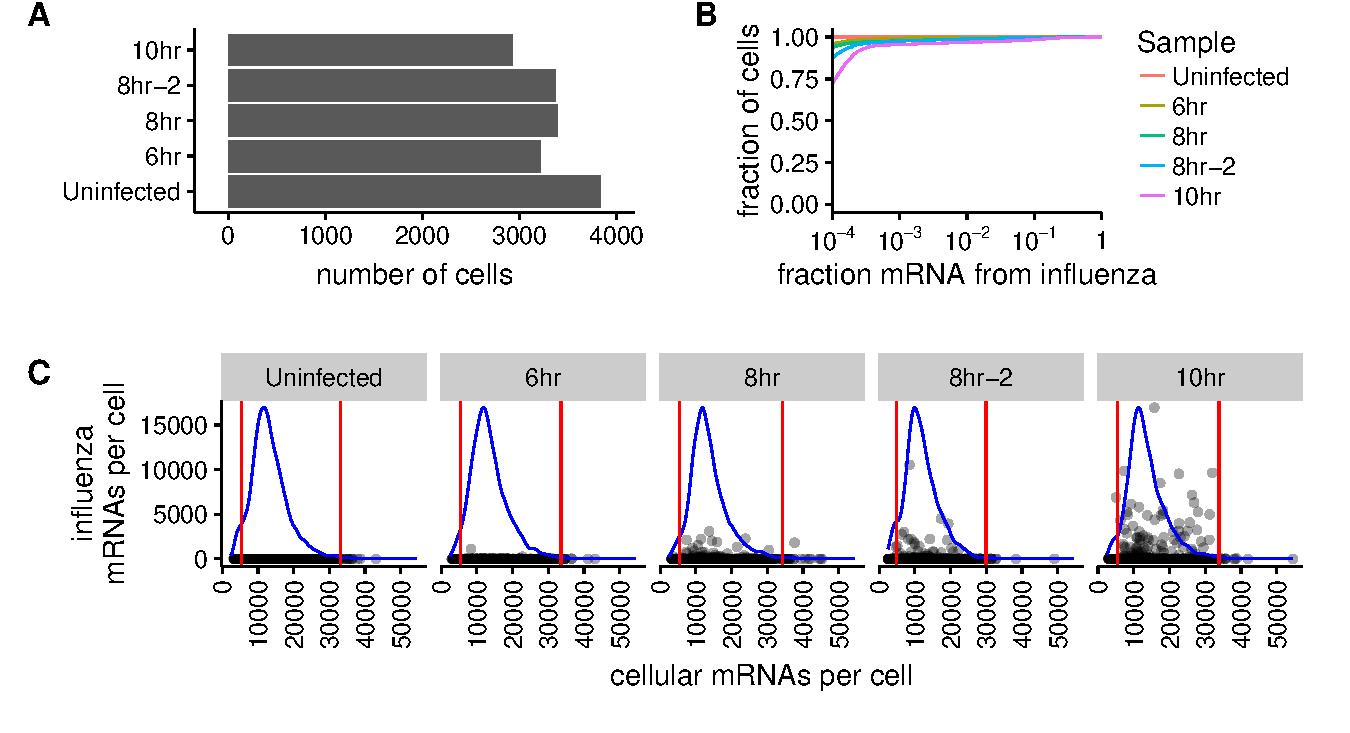
\includegraphics[width=0.9\linewidth]{figures/p_cell_mRNA_summary.pdf}}
\caption{\label{fig:cells}
There is a very wide distribution in the number of viral mRNAs detected per cell.
{\bf (A)} 
Number of cells sequenced for each sample.
{\bf (B)} 
Cumulative distribution of the fraction of mRNA derived from influenza virus for each sample.
For each point on the x-axis, the y-axis indicates the fraction of cells with at least that much of their mRNA from virus.
{\bf (C)} 
The number of cellular and viral mRNAs for each cell is plotted as a point.
The blue lines show the overall distribution of the number of cellular mRNAs per cell.
Cells outside the red lines were considered outliers (possibly derived from two cells per droplet), and were excluded from subsequent analyses.
}
\end{figure}

A complicating factor is that uninfected cells could have small amounts of viral mRNA due to leakage of transcripts from lysed cells.
It is therefore important to establish a threshold for identifying truly infected cells.
We can do this by taking advantage of the fact that roughly half the infecting virions bear synonymous barcodes.
Reads derived from lysed cells will be drawn from both wildtype and synonymously barcoded viral transcripts.
However, most cells are infected by at most one single virion, and so the reads from truly infected cells will usually derive almost entirely from one of the two viral variants. 
Figure~\ref{fig:viralbarcodes}A shows the fraction of viral reads in individual cells from each viral variant, and Figure~\ref{fig:viralbarcodes}B indicates the fraction of viral reads from the most abundant variant in that cell.
Most cells with a large amount of viral mRNA have viral transcripts exclusively derived from one viral variant -- indicating non-random partitioning as expected from viral infection.
However, cells with a small amount of viral mRNA often have viral transcripts from a mix of both variants, as expected from the random partitioning associated with simple mRNA leakage.
Finally, a few cells with a large amount of viral mRNA have viral transcripts from both variants, reflecting co-infection with both variants.

We determined the threshold amount of viral mRNA per cell at which the barcode partitioning clearly resulted from infection rather than leakage (Figure~\ref{fig:viralbarcodes}C), and used this threshold to annotate cells that we were confident were truly infected.
We also annotated as co-infected cells above this threshold that had mRNA from both viral variants.
Figure~\ref{fig:viralbarcodes}D shows the number of cells annotated as infected and co-infected for each sample -- these cells are just a small fraction of the number of cells with any viral read.
These annotation thresholds are conservative, and will miss some true low-level infections, as well as any co-infections with the same viral variant.
However, it is important that the analyses below are restricted to cells that are truly infected with virus, so we accepted the loss of some low-level infections in order to avoid false positives.
Because the bulk of cells are not infected, we subsampled the uninfected cells to the numbers shown in Figure~\ref{fig:viralbarcodes}D to balance the proportions of infected and uninfected cells for all subsequent analyses.

Strikingly, the extreme variation in the number of viral transcripts per cell remains even after we apply these rigorous criteria for annotating infected cells (Figure~\ref{fig:viralbarcodes}E). 
The fraction of viral mRNA per infected cell follows a roughly exponential distribution, with many cells having few viral transcripts and a few cells having many.
In fact, a bare few infected cells contribute the majority of influenza transcripts.
Specifically, at 6 and 8 hours $<$10\% of infected cells are responsible for over half the viral transcripts, while at 10 hours $\approx$15\% of infected cells produce over half the viral transcripts (Figure~\ref{fig:viralbarcodes}-Figure~supplement~\ref{figsupp:cumulfracflu}).

\begin{figure}[t!]
\centerline{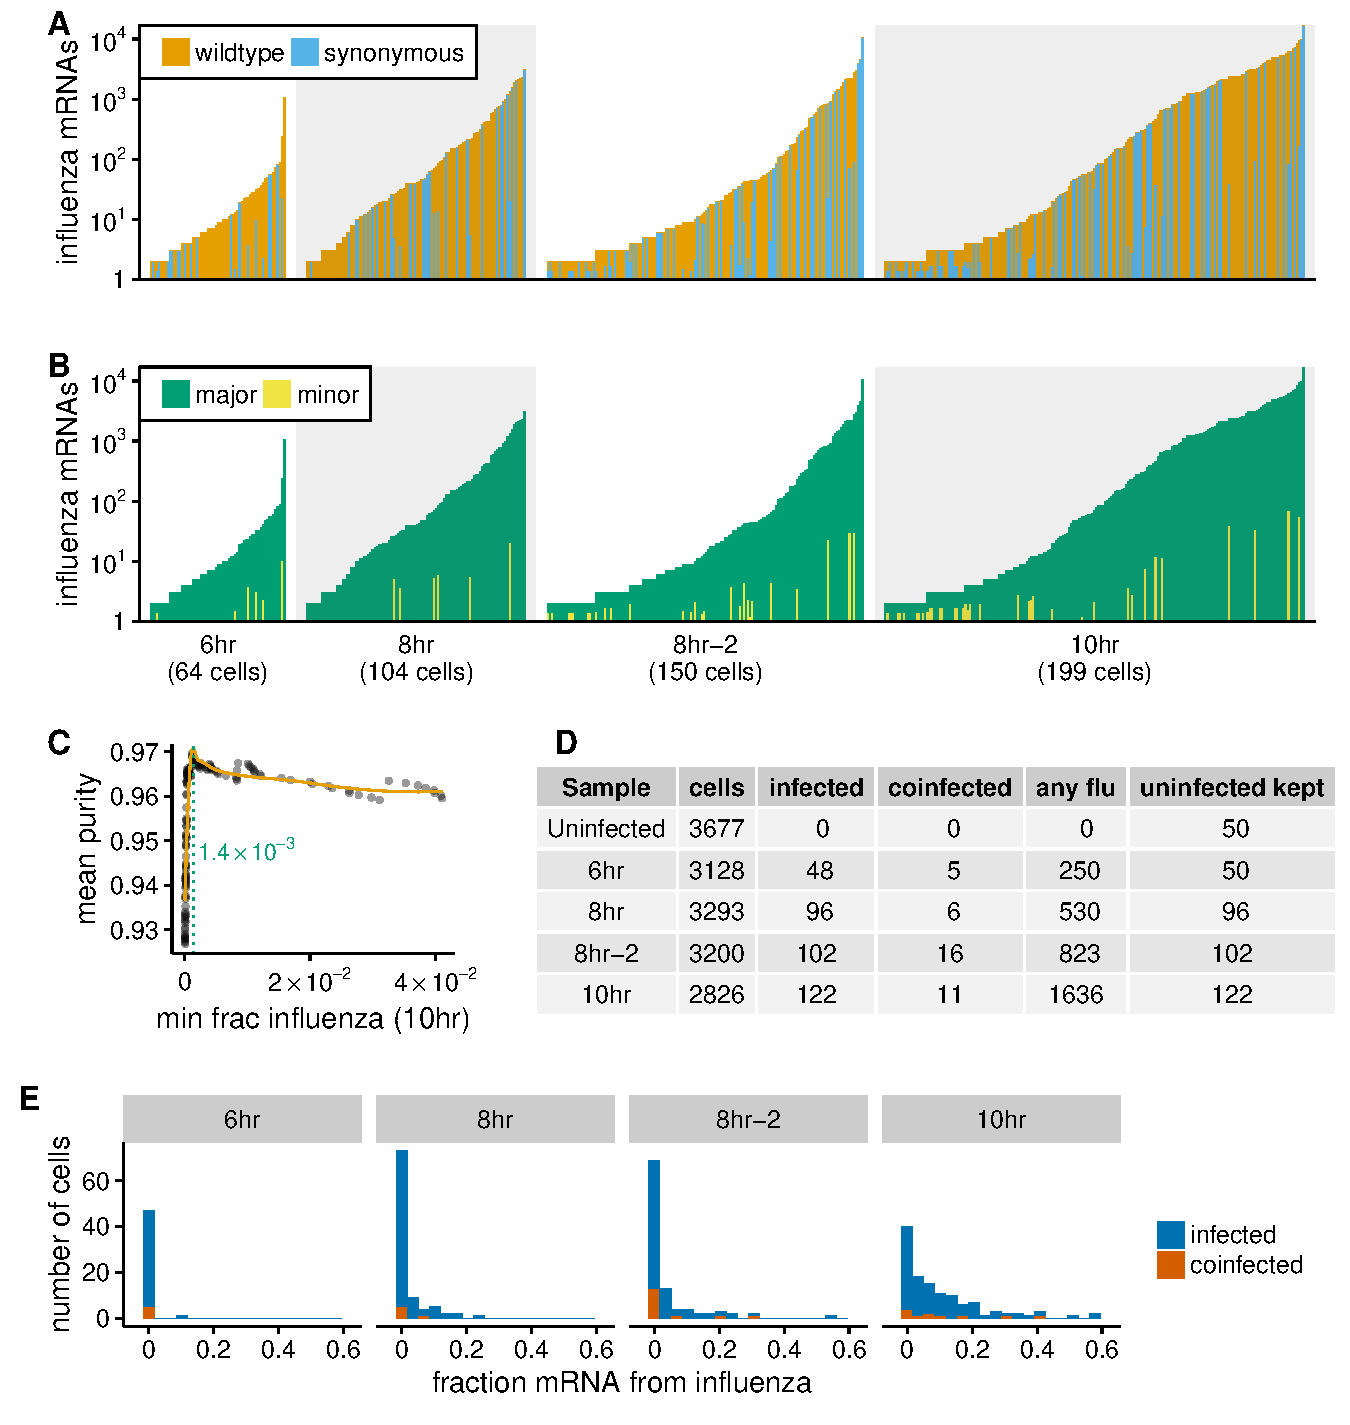
\includegraphics[width=0.9\linewidth]{figures/p_frac_flu_summary.pdf}}
\caption{\label{fig:viralbarcodes}
Synonymous barcodes on the viral mRNAs can help distinguish true infections from cells that contain viral mRNAs derived from leakage of lysed cells.
{\bf (A)}
Cells with at least two viral mRNAs for which the barcode could be called, arranged in order of increasing influenza transcript counts.
Bar heights denote the number viral mRNAs on a log\textsubscript{10} scale, bar coloring is linearly proportional to the fractions of viral mRNAs derived from wild-type and synonymously barcoded virus.
{\bf (B)}
Same as (A), but each bar is colored according to the relative fraction of the more common (major) and less common (minor) virus variant.
At low levels of viral mRNA there is often a roughly equal mix, suggesting contamination with viral mRNAs leaked from lysed cells.
At higher levels of viral mRNA, cells generally have only one viral variant, suggesting infection initiated by a single particle.
A few cells are also obviously co-infected with both viral variants.
{\bf (C)}
We determined a cutoff for calling ``true'' infections by fitting a curve to the mean barcode purity of all cells with greater than a given fraction of their mRNA derived from virus.
We called the cutoff at the point at which purity stops increasing with the fraction of viral mRNA.
{\bf (D)}
The number of cells identified as infected and co-infected for each sample, as well as the number of cells with any viral read.
For all subsequent analyses, we subsampled to a number of uninfected cells per sample to the greater of 50 or the number of infected cells.
{\bf (E)} 
Distribution of the fraction of mRNA per cell derived from virus for both infected and co-infected cells.
}
\figsupp[Number of viral barcodes called.\label{figsupp:barcodescalled}]{
The number of viral barcodes called for each sample and influenza gene segment. 
Viral transcripts are classified as \emph{syn} if they mapped to a synonymously barcoded influenza transcript, \emph{wt} if they mapped to a wild-type influenza transcript, \emph{invalid} if multiple reads for the same UMI differed on the status of the viral barcode, and as \emph{uncalled} if none of the reads for that UMI overlapped the region of the viral transcript containing the viral barcode.
}{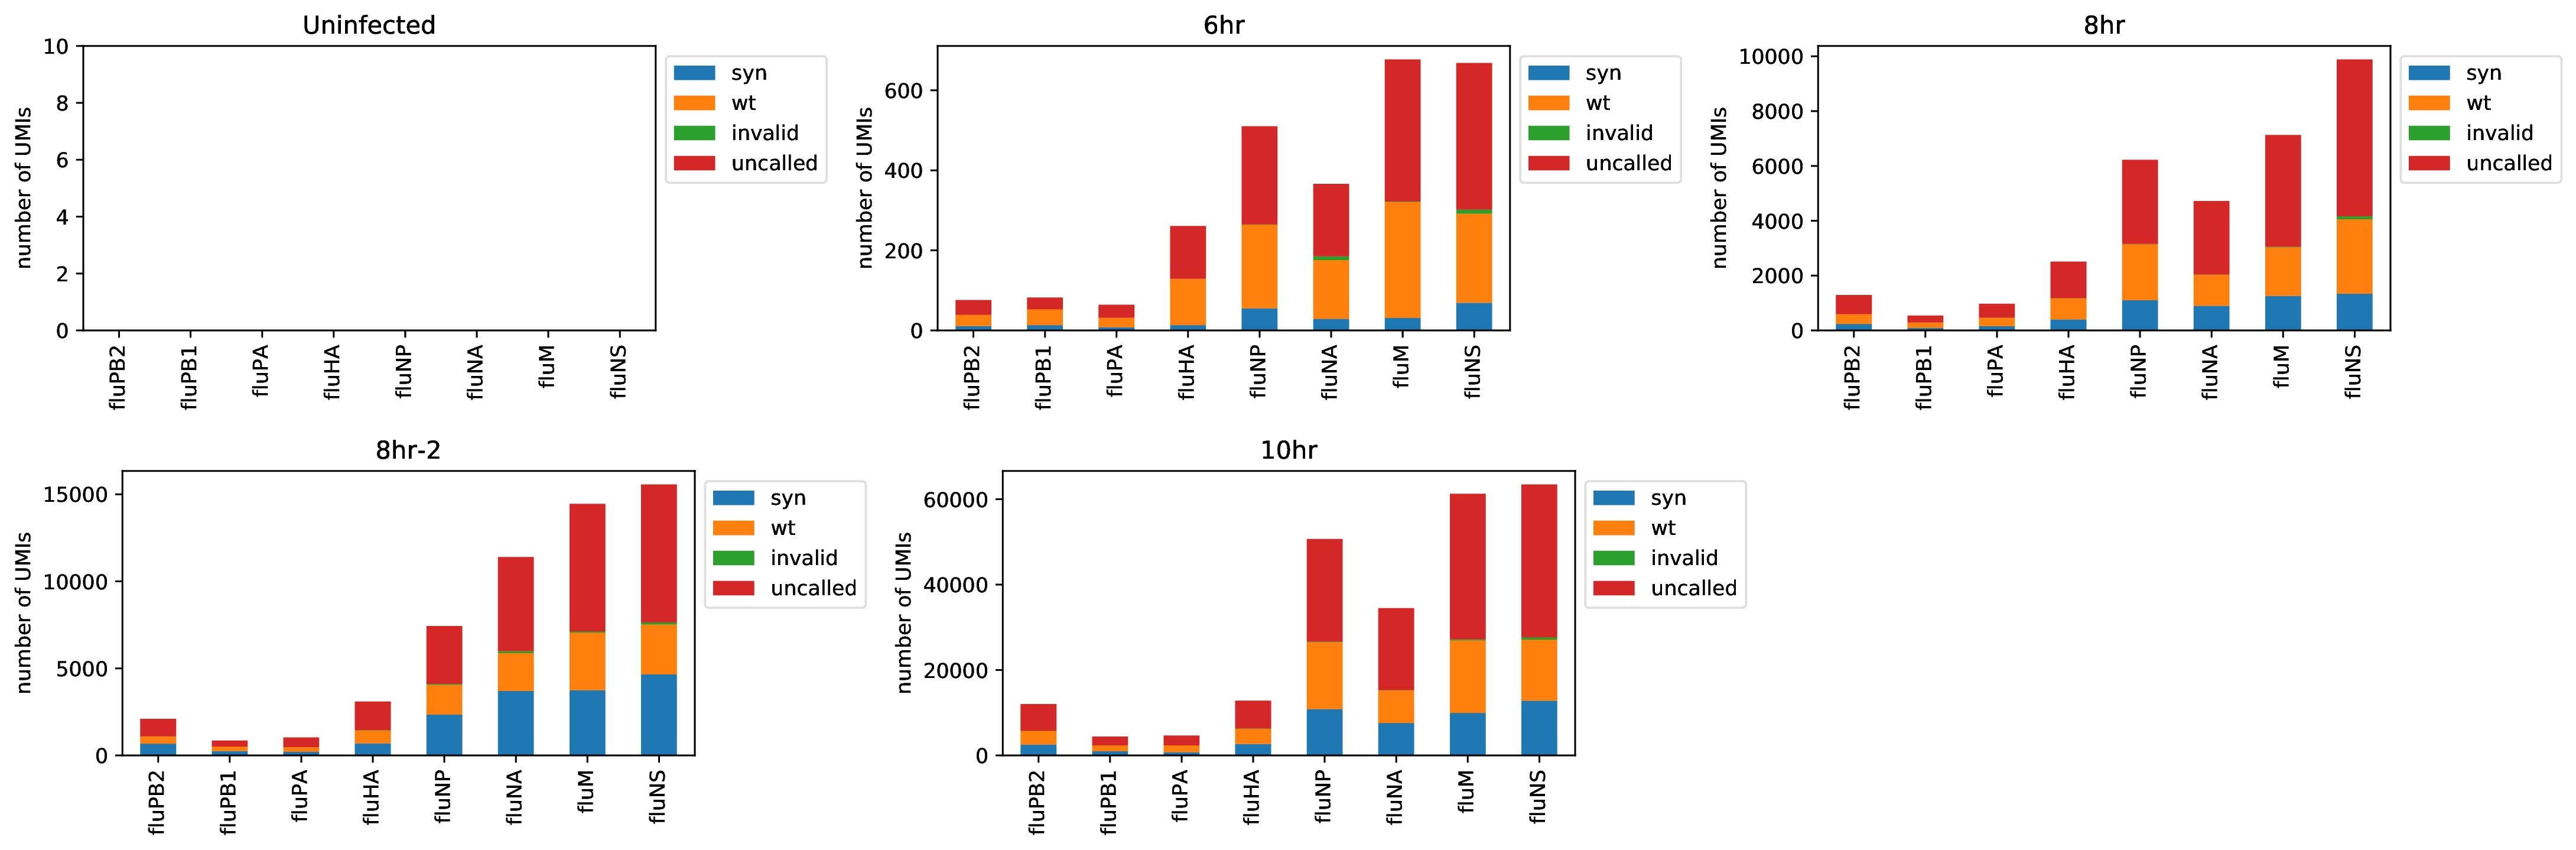
\includegraphics[width=\linewidth]{figures/synbarcodes_umistats.jpg}}
\figsupp[Fraction of total viral mRNA derived from a given fraction of infected cells.\label{figsupp:cumulfracflu}]{
The total fraction of all viral mRNA among infected cells that is attributable to a given fraction of these cells.
For instance, the plot for the 8-hour sample shows that roughly 50\% of all viral mRNA is derived from 10\% of the infected cells.
}{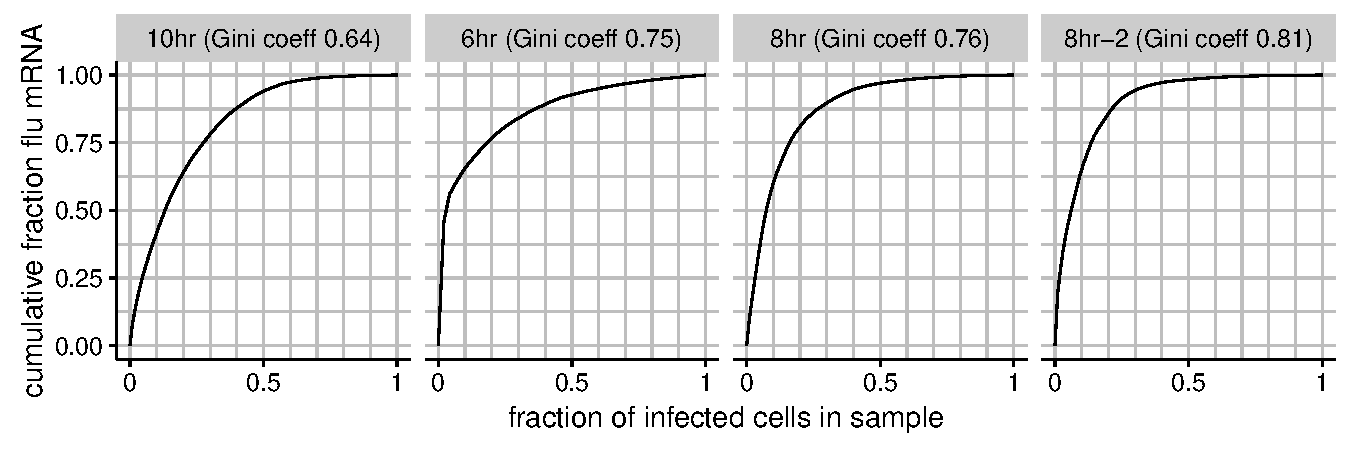
\includegraphics[width=\linewidth]{figures/p_cumul_flu.pdf}}
\end{figure}

\subsection{Absence of viral genes partially explains cell-to-cell variability in viral transcript abundance.}
The influenza genome is segmented, and cells can fail to express a viral mRNA if the encoding gene segment is not packaged in the infecting virion or fails to initiate transcription after infection.
Indeed, several groups have reported that the majority of infected cells fail to express at least one viral gene~\citep{brooke2013most}. 
We therefore wondered if the absence of specific viral genes might be associated with reduced amounts of viral mRNA within single infected cells.
In particular, transcription of influenza virus mRNAs is performed by the viral ribonucleoprotein (RNP) complex, which consists of the three proteins that encode the tripartite polymerase (PB2, PB1, and PA) as well as nucleoprotein (NP).
Each viral gene segment is associated with one RNP in the incoming infection virions, but secondary transcription by newly synthesized RNPs requires the presence of the viral genes that direct the synthesis of each of the four constituent RNP proteins.
This secondary transcription is a major source of viral mRNAs, as evidenced by the fact that blocking synthesis of the RNP proteins reduces the amount of viral mRNA by several orders of magnitude in bulk cells (Figure~\ref{fig:fluburdenbyflugene}-Figure~supplement~\ref{figsupp:cyclohexamide}).

\begin{figure}[t!]
\centerline{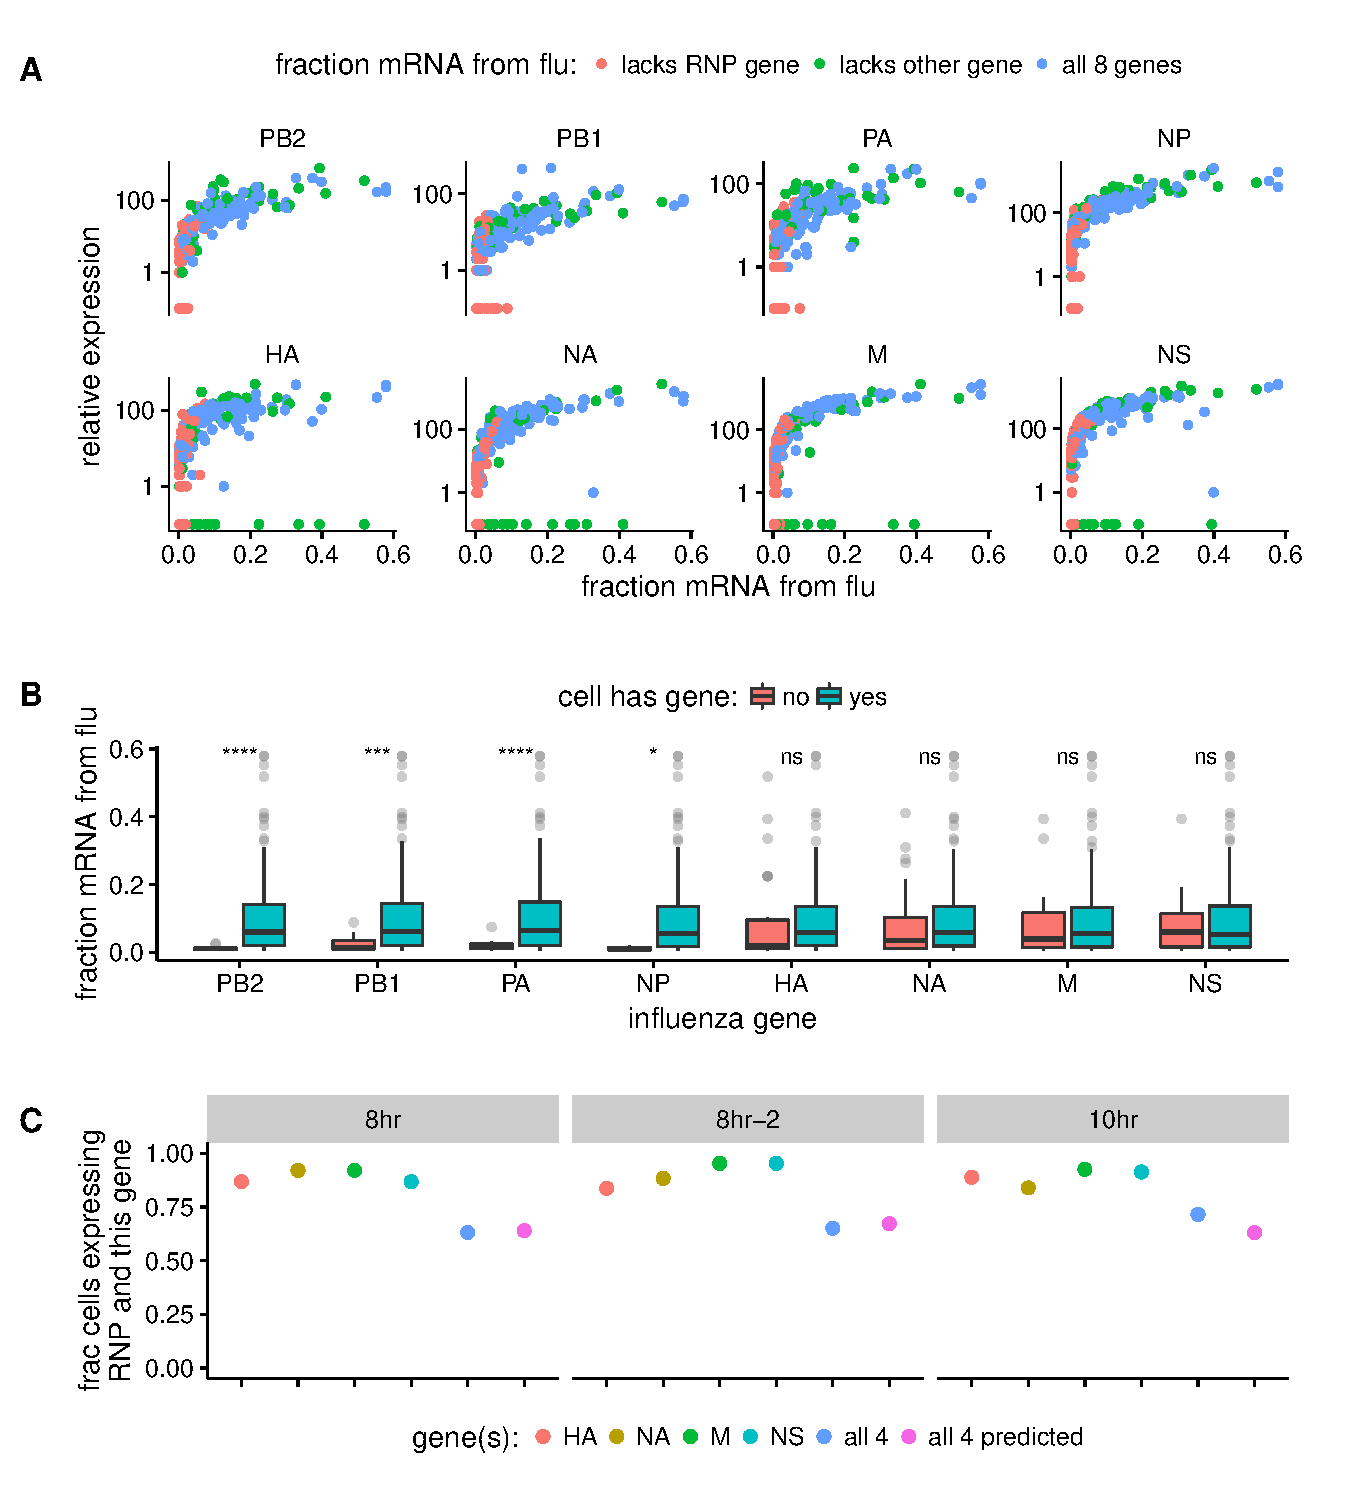
\includegraphics[width=0.9\linewidth]{figures/p_flu_burden_flu_gene_merge.pdf}}
\caption{\label{fig:fluburdenbyflugene}
The absence of viral genes explains some of the variability in the amount of viral mRNA per cell.
{\bf (A)} 
Fraction of mRNAs in each infected cell derived from virus as a function of the \emph{normalized} expression of each viral gene in that cell, taken over all time points.
Cells with high viral burden express all the RNP genes, but some cells with high viral burden lack each of the other viral genes.
{\bf (B)}
Box plots showing the per-cell viral burden among cells with $>$0.5\% of their mRNA from virus, binned by whether or not the cells express each viral gene.
A Wilcoxon signed-rank test was used to test the null hypothesis that absence of each gene does not affect viral burden: **** = $P < 10^{-4}$, *** = $P < 10^{-3}$,  * = $P < 0.05$.
Similar results are obtained if we examine only the 10-hour timepoint (Figure~\ref{fig:fluburdenbyflugene}-Figure~supplement~\ref{figsupp:10hrfluburdenbyflugene}).
{\bf (C)}
Fraction of infected cells that express all four RNP genes and also express each of the four other genes, as well as the fraction that express \emph{all} four of the other genes.
The fraction of cells that express all four of the other genes is well predicted by simply multiplying the frequencies of cells that express each of the four genes individually, indicating that the rate of segment absence is approximately independent across these four segments.
}
\figsupp[Secondary transcription from newly synthesized RNPs is a major source of viral mRNA during bulk infections.\label{figsupp:cyclohexamide}]{
A549 cells were infected at an MOI of 0.2 as calculated on MDCK-SIAT1 cels in either the presence or absence of the protein-translation inhibitor cyclohexamide, and viral mRNA was quantified at 8 hours post-infection by qPCR.
The cyclohexamide prevents translation of new PB2, PB1, PA, and NP protein, and so prevents the formation of the new RNPs needed for secondary transcription.
The bars show the relative amount of HA and PB2 mRNA in the absence versus the presence of cyclohexamide.
}{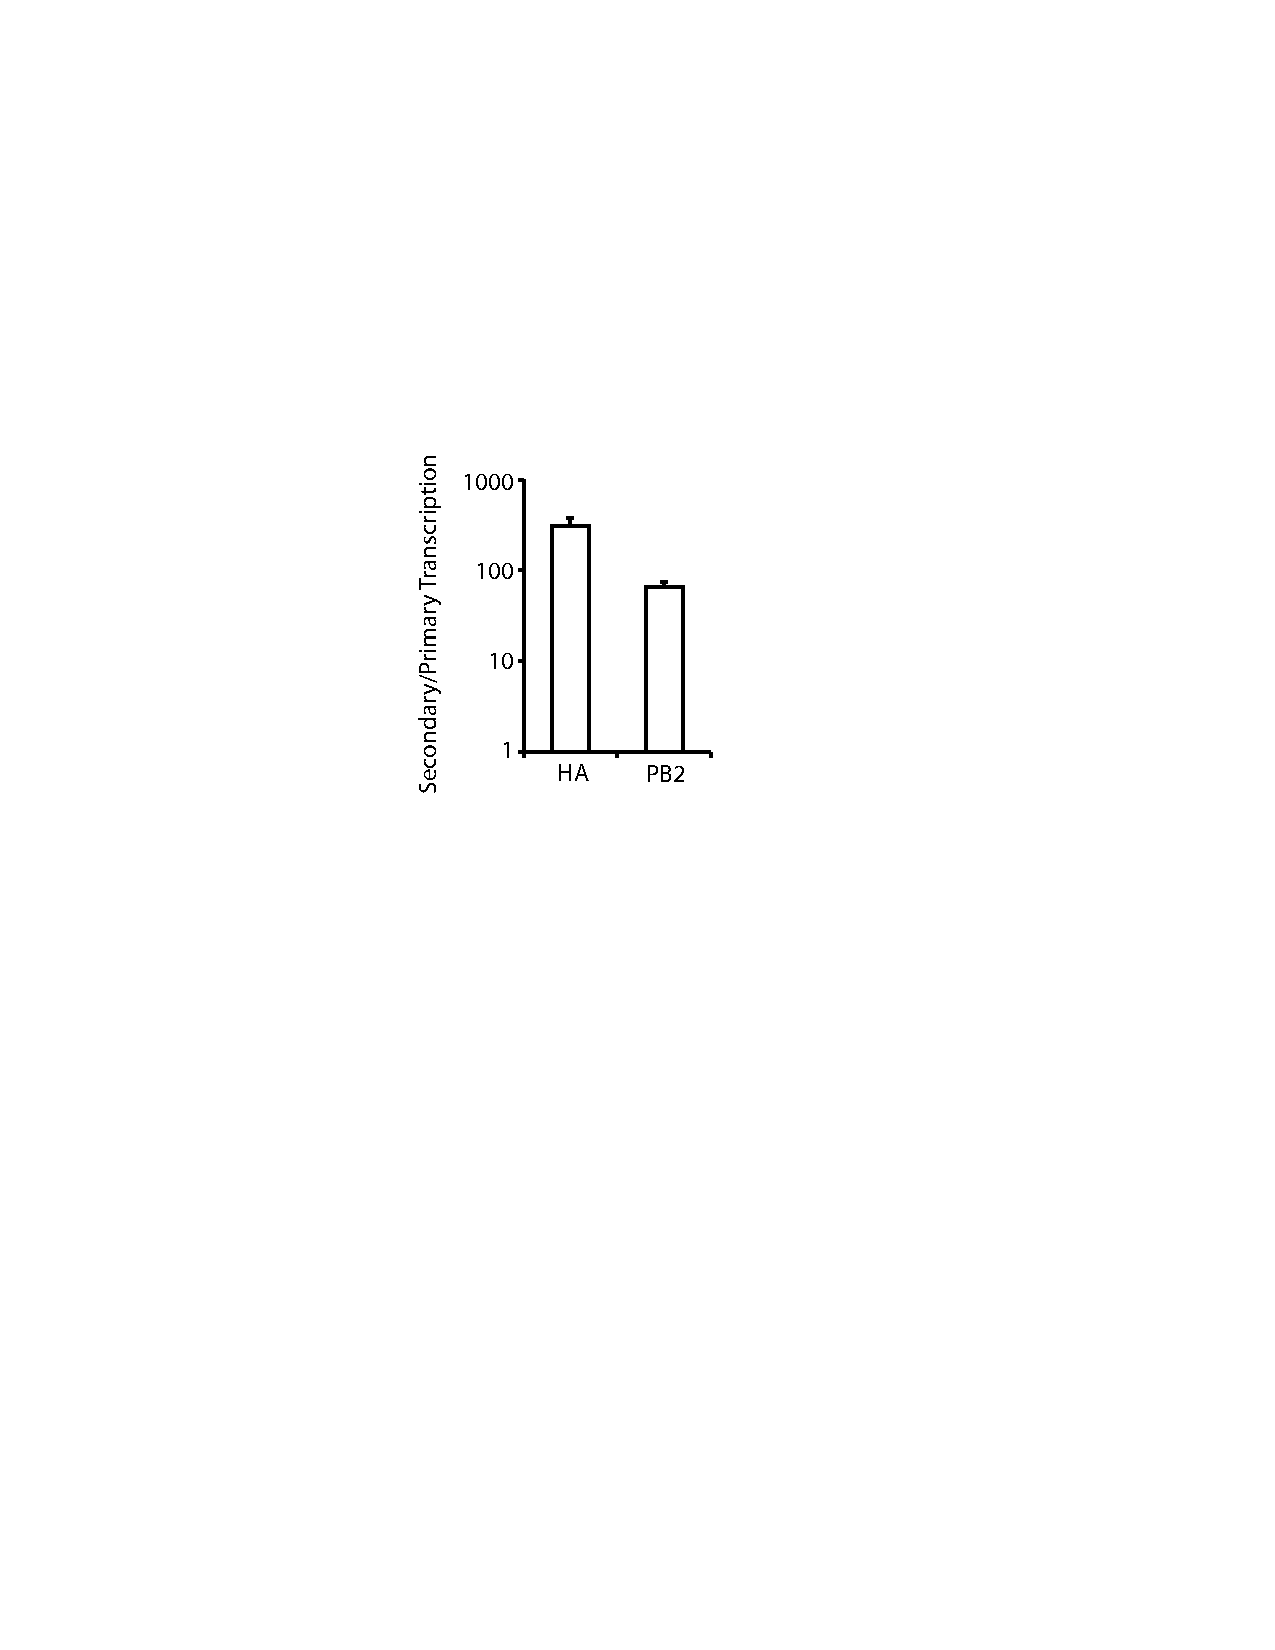
\includegraphics[width=0.3\linewidth]{figures/Primary_transcription_measurements/Cyclohexamide.pdf}}
\figsupp[Like panel (B) but for the 10-hr sample only.\label{figsupp:10hrfluburdenbyflugene}]{
The absence of viral RNP genes but \emph{not} non-RNP genes remains significantly associated with reduced viral burden when we examine only the 10-hr sample, which is the single time point with the most data points.
The difference for NP is no longer statistically significant due to low counts of infected cells lacking NP, but the trend remains.
}{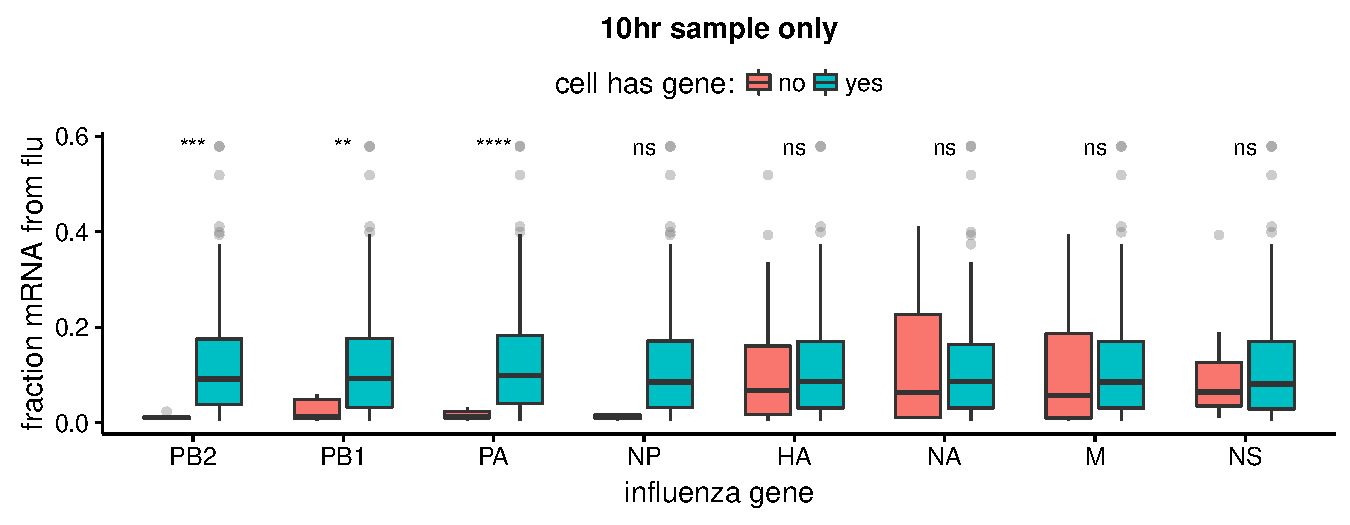
\includegraphics[width=\linewidth]{figures/p_10hr_flu_burden_flu_gene_test}}
\figdata{The numerical data for panel (C) are in \texttt{p\_missing\_genes.csv}.}
\end{figure}

We examined the total fraction of mRNA in each cell that derives from virus versus the relative expression of each viral gene in that cell (Figure~\ref{fig:fluburdenbyflugene}A). 
Cells that lack one of the RNP genes never derive more than a few percent of their mRNAs from virus, demonstrating that the presence of these RNP genes are essential for high levels of viral transcription.
However, we observe cells that lack each of the other non-RNP genes but still derive $\approx$40\% of their mRNAs from virus, suggesting that none of the other genes are important for high levels of viral transcription.
These results are statistically supported by the analysis in Figure~\ref{fig:fluburdenbyflugene}B, which shows that absence of any of the four RNP genes but \emph{not} any of the other viral genes is associated with reduced amounts of viral mRNA. 
However, gene absence clearly does not explain all of the variability in viral gene expression, since even cells expressing all eight segments exhibit a very wide distribution in the number of viral mRNAs that they express. 
Additional mechanisms, such as differences in host-cell state or viral mutations not detectable by our 3'-end sequencing approach, must explain the remainder of this variability.  

We also sought to quantify the fraction of infected cells that completely failed to express a given gene.
We limited this analysis to examining the presence / absence of the non-RNP genes in cells expressing all four RNP genes, since we might fail to detect viral transcripts that are actually present at low levels in RNP-deficient cells due to the lower viral burden in these cells.
At the 8- and 10-hour time points, between 5\% and 17\% of cells fail to express any one of the four non-RNP genes (Figure~\ref{fig:fluburdenbyflugene}C).
The absence of a given segment appears to be an independent event, as the probability of observing all four non-RNP segments in a cell is well predicted by simply multiplying the probabilities of observing each of the four segments individually (Figure~\ref{fig:fluburdenbyflugene}C). 
These numbers on the frequency at which infected cells fail to express individual viral genes are roughly consistent with measurements made by others using different means~\citep{brooke2013most}.
	
\subsection{Despite variability in absolute abundance, relative amounts of influenza mRNAs are comparatively constrained}
	
In contrast to our analyses above, the fraction of influenza mRNAs derived from a given segment behaves in a more stereotyped fashion -- regardless of how many influenza transcripts are observed in a given cell (Figure ~\ref{fig:fluexpr}A).
Rather than the several order of magnitude degree of variance observed in influenza mRNA abundance, the inter-quartile range of influenza ratios observed tends to be relatively tight, clustered around a median value consistent with prior population-level measurements (Figure ~\ref{fig:fluexpr}B).
The greatest degree of variance between the first and third quartile of any segment in our analysis only exhibited a \textasciitilde3-fold range.
These values appear consistent whether or not we limit the analysis to only those cells expressing all eight segments (Figure ~\ref{fig:fluexpr}C,D).
Therefore while either noise in influenza replication or host variability can dramatically impact the amount of influenza mRNA produced as a whole, these processes seem to, ignoring complete absence of a segment, act equally across the influenza genome.
This is consistent with more limited experiments showing positive correlations between several segments in vRNA measurements in single cells.
Therefore it can be inferred that the process by which influenza generates relative mRNA abundances is robust to the noise inherent in infection, or at least significantly more so than those processes that drive total mRNA abundance.

\begin{figure}
\centerline{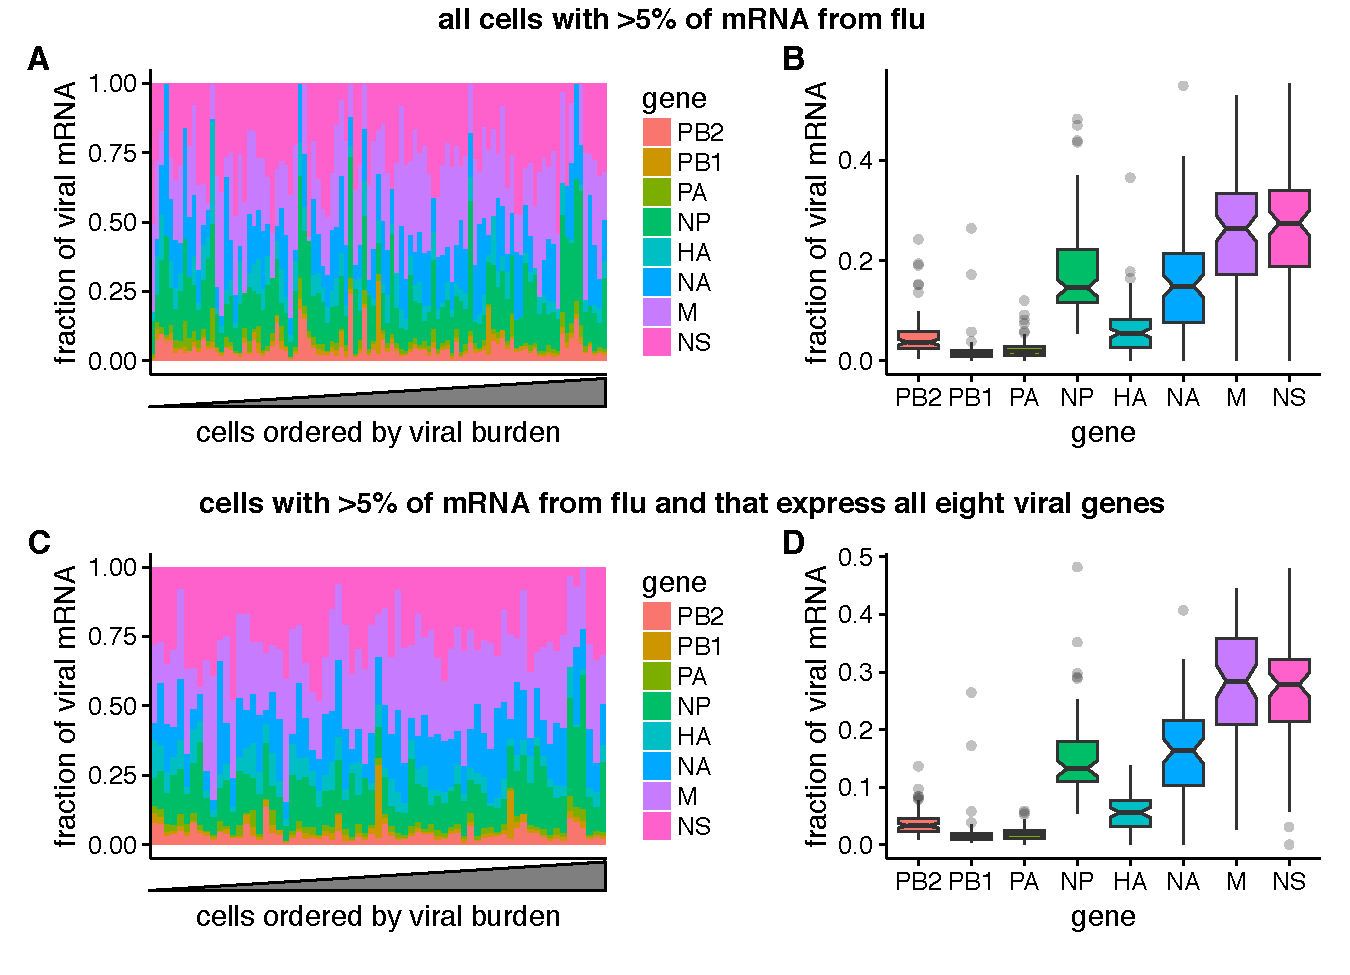
\includegraphics[width=0.9\linewidth]{figures/p_flu_expr_aledit.pdf}}
\caption{\label{fig:fluexpr}
Expression of individual influenza genes in highly infected cells (at least 5\% of total mRNA is viral).
{\bf (A)} 
The fraction of total mRNA from each influenza gene for each cell. 
{\bf (B)}
Box plots showing the fraction of viral mRNA per cell that is derived from each influenza gene taken over all highly expressed cells.
The black line at the notch in each box is the median, and the top and bottom of the box indicate the first and third quartiles.
{\bf (C,D)} As in {\bf(A,B)} save only for cells in which all eight gene segments are observed.
}
\figdata{The raw data are in \texttt{p\_flu\_expr.csv}.}
\end{figure}

\subsection{Co-infection potentially increases successful viral infections}
While relatively rare in our dataset, those cells positively identified as containing both wild-type and synonymously barcoded influenza provide important insight into the nature of co-infection. 
It has been posited that co-infection can rescue infections missing one or more segments, potentially by providing missing genome equivalents.
\emph{Brooke et al}, for example observed increased co-occurrence of a given gene-segment pair as MOI was increased. 
Consistent with this model, we frequently observe a single barcode for a given gene segment, suggesting it was only provided by one virion (Figure ~\ref{fig:coexpression}).
This interpretation does however, make the assumption that absence is not instead driven by competition between segments.
When we examine our co-infected cells, we observe a higher rate of co-expression of the four non-RNP segments than calculated above (80\% as compared to 63-70\%), with the caveat that this is an incredibly small sample size to draw from.
Another observation that can be immediately procured is that, on the whole, co-infections have roughly balanced amounts of wild-type and barcoded segments. 
Others have noted that windows for co-infection are relatively narrow, and, these data suggest that the co-infections we observe likely occurred before significant genome replication -- a process which would dramatically advantage the earlier virion.
To support these conclusions using a larger dataset, we generated a virus in which the HA segment was replaced by GFP, allowing us to detect co-infection by both wild-type and mutant virus by flow cytometry (Figure ~\ref{fig:flowcyto}A).
When we examine strictly co-infected cells, we observe that, as in our single-cell analysis, both HA and GFP are highly correlated -- indicating a tight window of co-infection (Figure ~\ref{fig:flowcyto}B).
Moreover, a portion of the population expressing only low HA, which likely includes those viruses only engaging in primary transcription, is greatly reduced, suggesting rescue of this phenotype by co-infection (Figure ~\ref{fig:flowcyto}C). 
These data give credence to the sentiments of others that co-infection may be a significant contributor to influenza pathogenesis.

\begin{figure}
\centerline{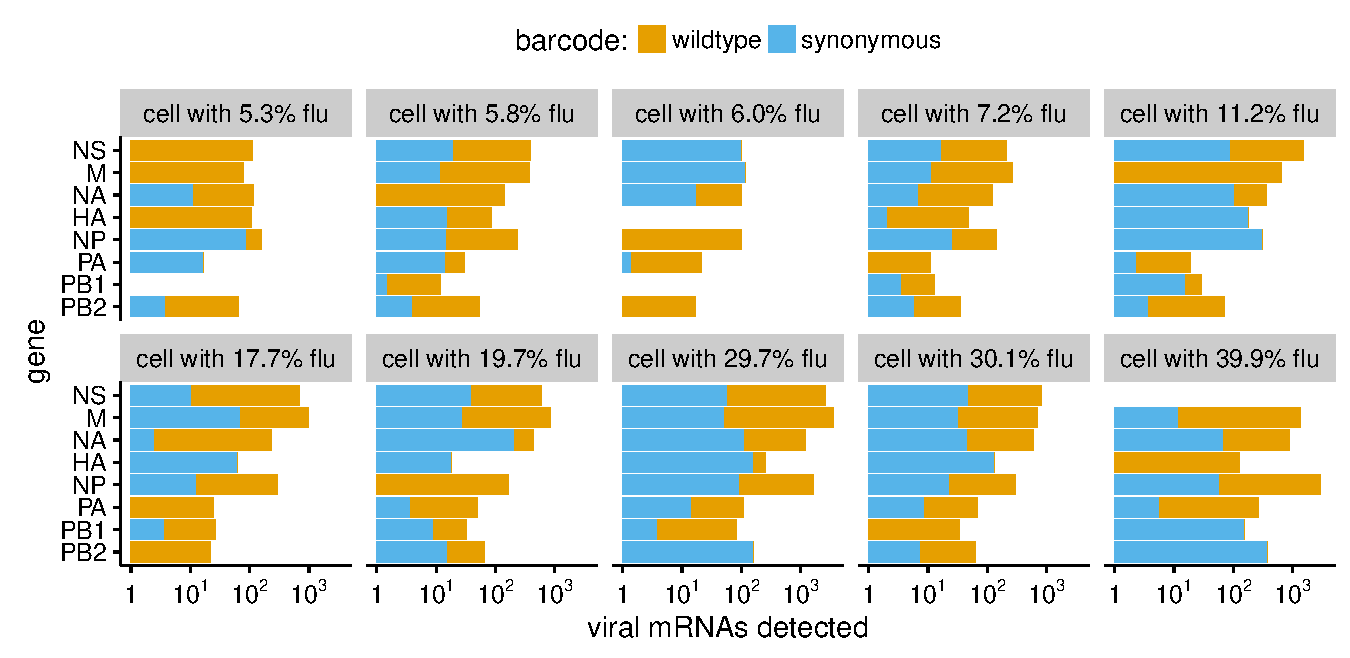
\includegraphics[width=0.9\linewidth]{figures/p_coinfection.pdf}}
\caption{\label{fig:coexpression}
Frequency of each viral gene segment in co-infected cells with at least 5\% of their mRNA derived from influenza.
The bars indicate the logarithm of the number of each viral mRNA detected, and the bars are colored in proportion to the fraction of those mRNAs that are derived from either wildtype or synonymous barcoded virus.
}
\figdata{The raw data plotted in this figure are in \texttt{p\_co-infection.csv}.}
\end{figure}

\begin{figure}
\centerline{\includegraphics[width=0.9\linewidth]{figures/Pseudovirus_flow_cytometry/coinfFlow_D01.pdf}}
\caption{\label{fig:flowcyto} Co-infection occurs relatively early and potentially provides an advantage. 
{\bf(A)} Cells were infected with wild-type virus and a virus in which HA has been replaced by eGFP at an MOI of 0.1 of each virus as calculated on MDCK-SIAT1 cells or MDCK-SIAT1 cells expressing HA, respectively.
Cells were stained for HA and additionally analyzed for eGFP expression at 10h post infection. Full flow cytometric analysis shown.
{\bf(B)} HA and eGFP signal are correlated in co-infected cells. Quantile-normalized HA and eGFP signal for those cells identified as eGFP\textsuperscript{+} HA\textsuperscript{+}. Cells colored by density, using a Gaussian kernel density estimate. 
{\bf(C)} Low-HA cells are reduced in co-infections. Guassian density estimates for HA signal in HA\textsuperscript{+} cells either expressing or failing to express eGFP. 
{\bf(D)} Uninfected control used to set gates for {\bf(A)}
}
\figsupp[Additional replicates and gating controls.\label{}]{
}{\includegraphics[width=\linewidth]{}}
\end{figure}

\subsection{Identifying host features of influenza infection}
Single cell measurements not only allow us to observe heterogeneity with respect to progression through a process, but also to capture cell states of subpopulations within complex mixtures.
Measurements of the host response to influenza have been confounded by the complexity of the infectious process, and, therefore, are predominated by those processes with the greatest differential of expression, regardless of the prevalence of response in the population or their specific association with infection state.
To begin to understand the cellular response to influenza, or, alternatively, influenza remodeling of the cellular state, we first needed to understand whether transcriptomes of influenza-infected cells could be distinguished from their uninfected counterparts. 
We therefore undertook tSNE analysis to determine whether influenza drives changes in transcriptomic state above-and-beyond between-cell variability independent of infection. 


\subsection{Influenza infection is associated with the antioxidant response}

\begin{figure}
\centerline{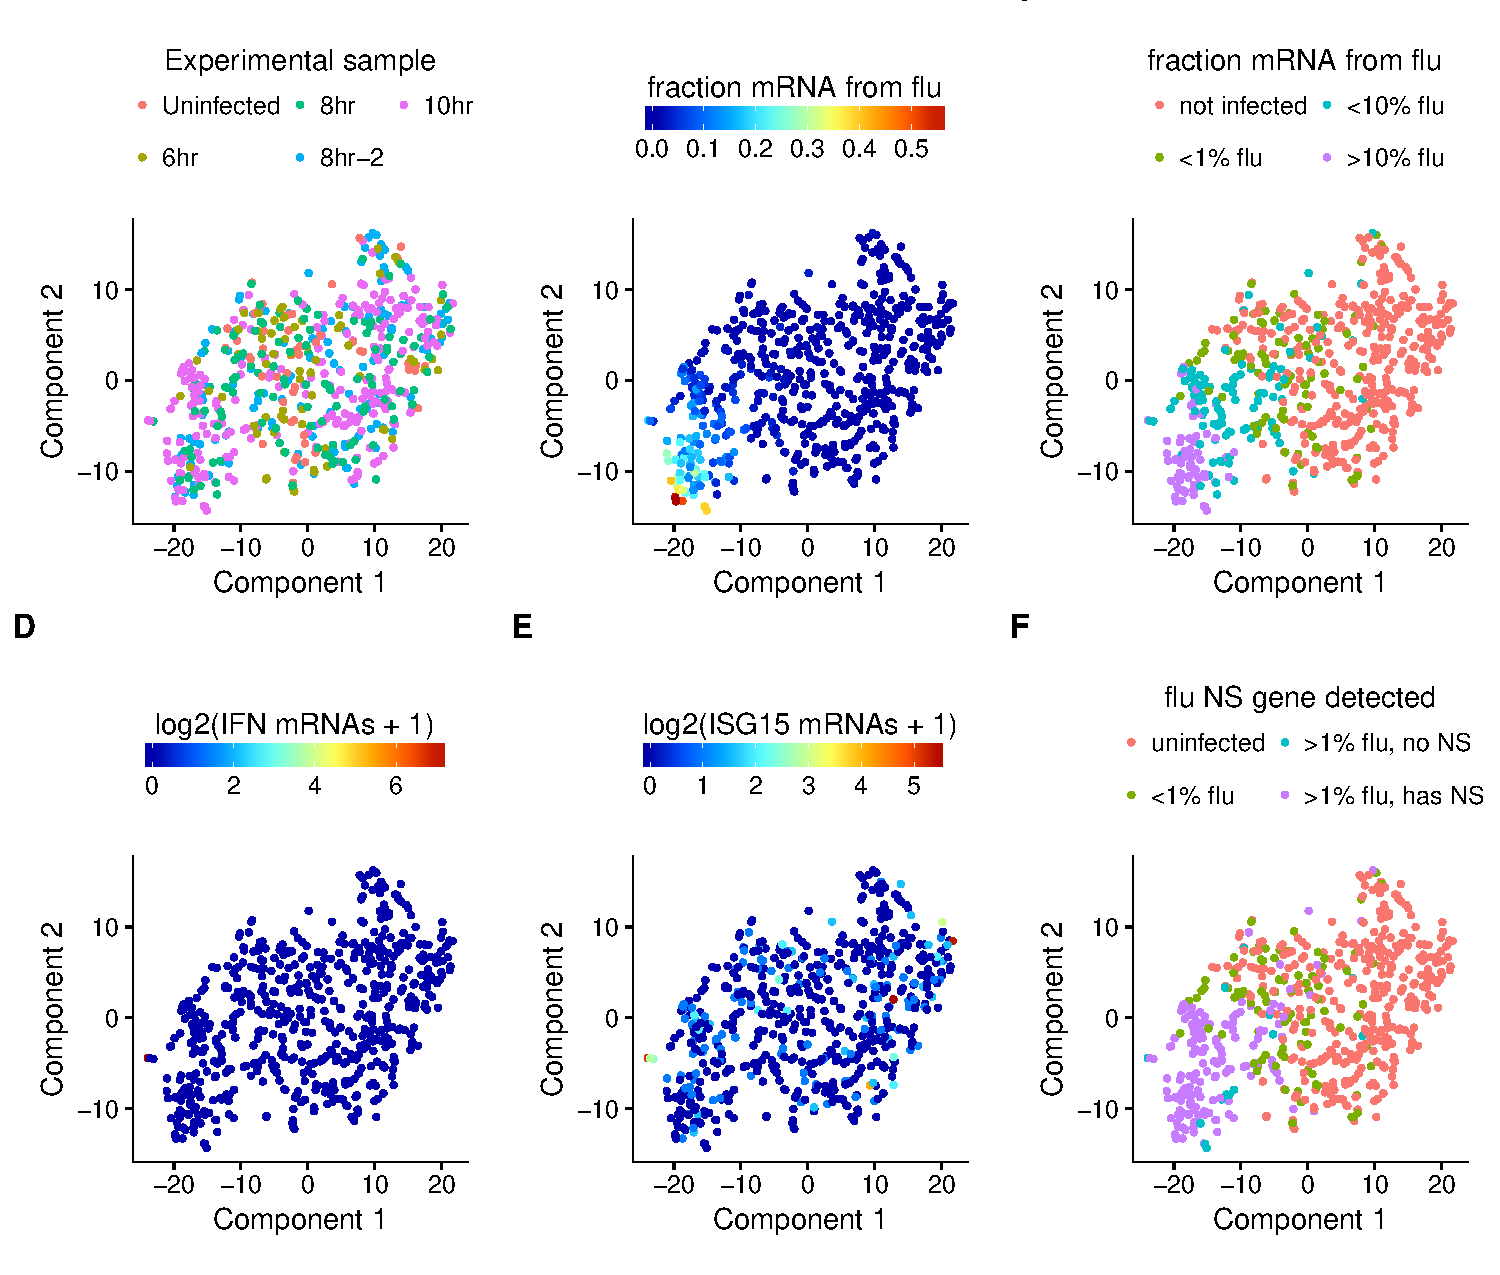
\includegraphics[width=0.9\linewidth]{figures/p_small_tsne_merge.pdf}}
\caption{\label{fig:tsne}
tSNE plots.
The layout is the same in all panels, but each panel colors the cells according to a different property.
{\bf (A), (B)}
Cells colored by the fraction of their mRNA that is viral.
{\bf (C)}
Cells colored by experimental sample.
While it is clear that cells from later timepoints often have more viral RNA, there are cells from earlier timepoints with a high viral burden and cells from late timepoints with a low viral burden.
{\bf (D)}
Cells colored by the number of type I and III interferon transcripts detected.
Only one cell has high expression of these interferons.
{\bf (E)}
Cells colored by the expression of the interferon-stimulate gene ISG15.
{\bf (F)}
For cells with at least 1\% of their reads from influenza, are the cells expressing the viral NS protein?
The one interferon-positive cell is lacking NS, but many other cells also lack NS but do not express interferon.
}
\end{figure}


\begin{figure}
\centerline{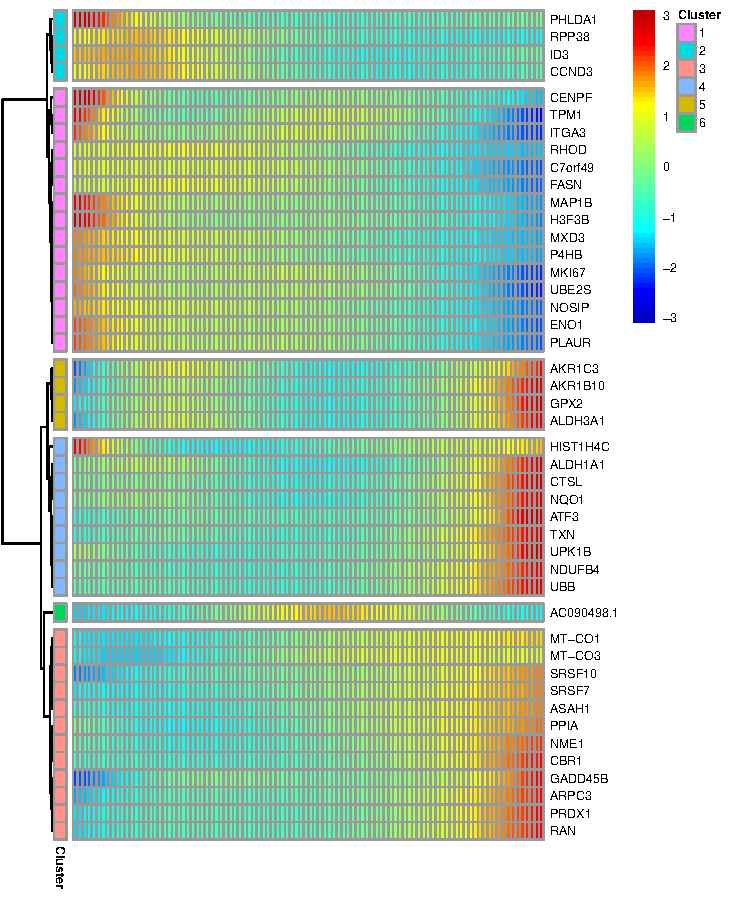
\includegraphics[width=0.8\linewidth]{figures/p_cellular_heatmap.pdf}}
\caption{\label{fig:cellulargenes}
Cellular genes that are differentially expressed with respect to the amount of influenza mRNA in individual cells infected with full influenza virus containing all eight genes.
Shown are all genes differentially expressed with $Q < 0.1$.}
\figdata{The full results of the differential expression test is in \texttt{p\_sig\_cellular\_genes.csv}.}
\figdata{The results of a gene-set analysis are in \texttt{p\_sig\_cellular\_genes.csv}.}
\end{figure}

\section{Discussion}

\lipsum[9]

\section{Methods and Materials}

Guidelines can be included for standard research article sections, such as this one. 

\lipsum[3]

\section{Some \LaTeX{} Examples}
\label{sec:examples}

Use section and subsection commands to organize your document. 
\LaTeX{} handles all the formatting and numbering automatically. 
Use ref and label commands for cross-references.

\subsection{Figures and Tables}


If you use the following prefixes for your \verb|\label|:
%
\begin{description}
\item[Figures] \texttt{fig:}, e.g.~\verb|\label{fig:view}|
\item[Tables] \texttt{tab:}, e.g.~\verb|\label{tab:example}|
\item[Equations] \texttt{eq:}, e.g.~\verb|\label{eq:CLT}|
\item[Boxes] \texttt{box:}, e.g.~\verb|\label{box:simple}|
\end{description}
%
you can then use the convenience commands as in \verb|\FIG{cells}|, \ to generate cross-reference \FIG{view}. 

\subsection{Citations}

LaTeX formats citations and references automatically using the bibliography records in your .bib file, which you can edit via the project menu. 
Use the \verb|\cite| command for an inline citation, like \cite{trapnell2014pseudo}, and the \verb|\citep| command for a citation in parentheses \citep{trapnell2014pseudo}. 
The LaTeX template uses a slightly-modified Vancouver bibliography style. 
If your manuscript is accepted, the eLife production team will re-format the references into the final published form. 
\emph{It is not necessary to attempt to format the reference list yourself to mirror the final published form.}


\section{Acknowledgments}

Additional information can be given in the template, such as to not include funder information in the acknowledgments section.

\nocite{*} % This command displays all refs in the bib file
\bibliography{references}


\end{document}
ommand displays all refs in the bib file
\bibliography{references}


\end{document}
ent}
{document}
 This command displays all refs in the bib file
\bibliography{references}


\end{document}
ommand displays all refs in the bib file
\bibliography{references}


\end{document}
 refs in the bib file
\bibliography{references}


\end{document}
ommand displays all refs in the bib file
\bibliography{references}


\end{document}
iography{references}


\end{document}
ent}
eferences}


\end{document}
ent}
